\documentclass[a4paper,10pt]{article}
\usepackage[catalan]{babel}
\usepackage[utf8x]{inputenc}
\usepackage{amsmath}
\usepackage{amsfonts}
\usepackage{amssymb}
\usepackage{amsthm}
\usepackage{graphicx}


\title{Memòria pràctica 8}
\author{Josep Marc Mingot//, 
      Gabriel Reines}
      
%%%%%%%%%%%%%%%%%%%%%%%%%%%%%%%%%%%%%%%%%%%%%%%%%%%%%%%%%%%%%%%%%%%%%%%%%%%%%%%%%%%%%%%%%%%%%%%%%%%
\usepackage{Sweave}
\begin{document}
\Sconcordance{concordance:memoria.tex:memoria.Rnw:%
1 15 1 1 0 1 4 34 1 1 4 6 1 1 4 38 1 1 2 15 0 1 2 15 1 1 2 16 0 1 2 1 1 1 5 6 1 1 4 6 1 1 4 25 1 1 4 6 1 1 4 6 1 1 4 40 1}



\maketitle

\begin{abstract}
\end{abstract}

\newpage
\tableofcontents

\newpage
%%%%%%%%%%%%%%%%%%%%%%%%%%%%%%%%%%%%%%%%%%%%%%%%%%%%%%%%%%%%%%%%%%%%%%%%%%%%%%%%%%%%%%%%%%%%%%%%%%%
\section{Introducció}

In this example we embed parts of the examples from the
\texttt{kruskal.test} help page into a \LaTeX{} document:
\begin{Schunk}
\begin{Sinput}
> data(airquality)
\end{Sinput}
\end{Schunk}
which shows that the location parameter of the Ozone 
distribution varies significantly from month to month. Finally we
include a boxplot of the data:



%%%%%%%%%%%%%%%%%%%%%%%%%%%%%%%%%%%%%%%%%%%%%%%%%%%%%%%%%%%%%%%%%%%%%%%%%%%%%%%%%%%%%%%%%%%%%%%%%%%
\section{Visualització de dades}

El primer pas en qualsevol problema de classificació és entendre les dades que se'ns han donat. Per aquest motiu en aquesta secció pretenem donar a través de l'anàlisi visual, una serie de propietats sobre les variables que influeixen en el problema.
\\
\\
Comencem estudiant la correlació entre elles. Al tenir 116 variables l'eina més adequada per visualitzar l'autocorrelació entre elles és visualitzar gràficament la matriu de correlació. En la figura \ref{fig:autoc} observem la matriu on cada casella representa un valor i com més fosc més proper a 1. Hi ha variables que estan completament correlacionades (per exemple \texttt{neighborhood intensity feature 2} amb \texttt{neighborhood intensity feature 8}). Per eliminar-les, fixem un nivell a partir del qual considerem que les variables estan correlacionades i n'eliminem aquella que té una mitja de correlació més alta amb les altres. Després d'aquest procés i fixant un tall a 0.85 passem de 116 variables a 88 variables. Podem observar la matriu d'autocorrelació neta en la figura \ref{fig:autoc_clean}.



\begin{center}
\begin{figure}
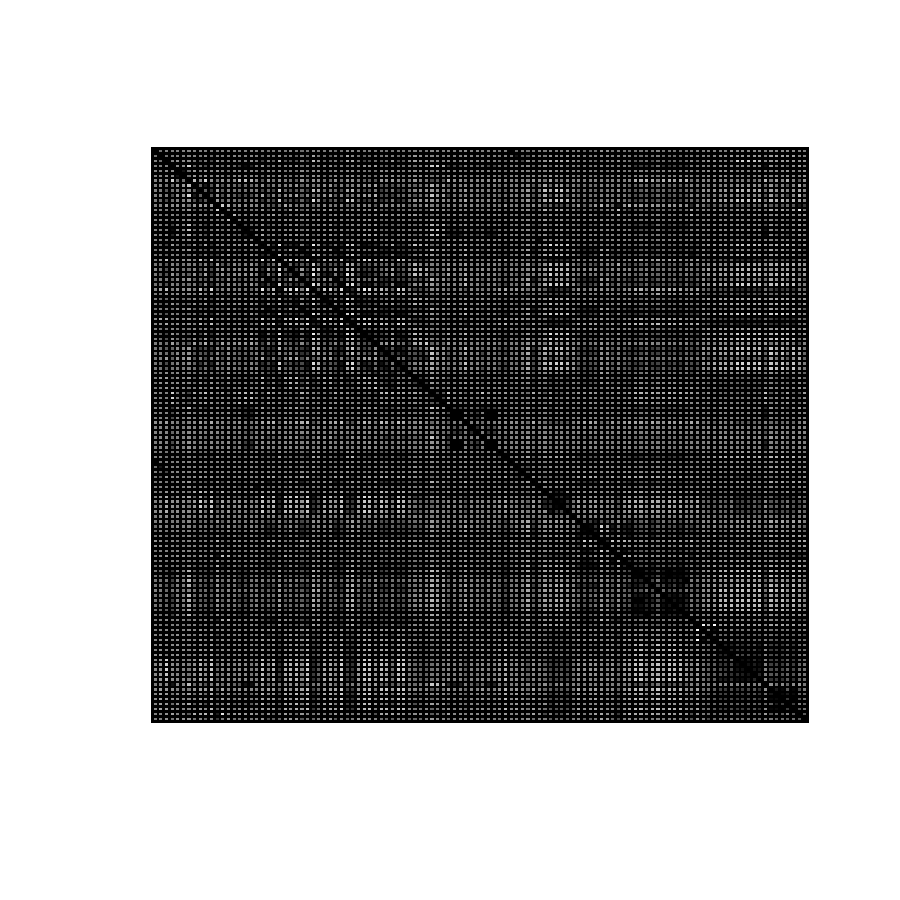
\includegraphics[width=5in]{memoria-autoc}
\caption{Autocorrelació de les 117 variables.} \label{fig:autoc}
\end{figure}
\end{center}

\begin{center}
\begin{figure}
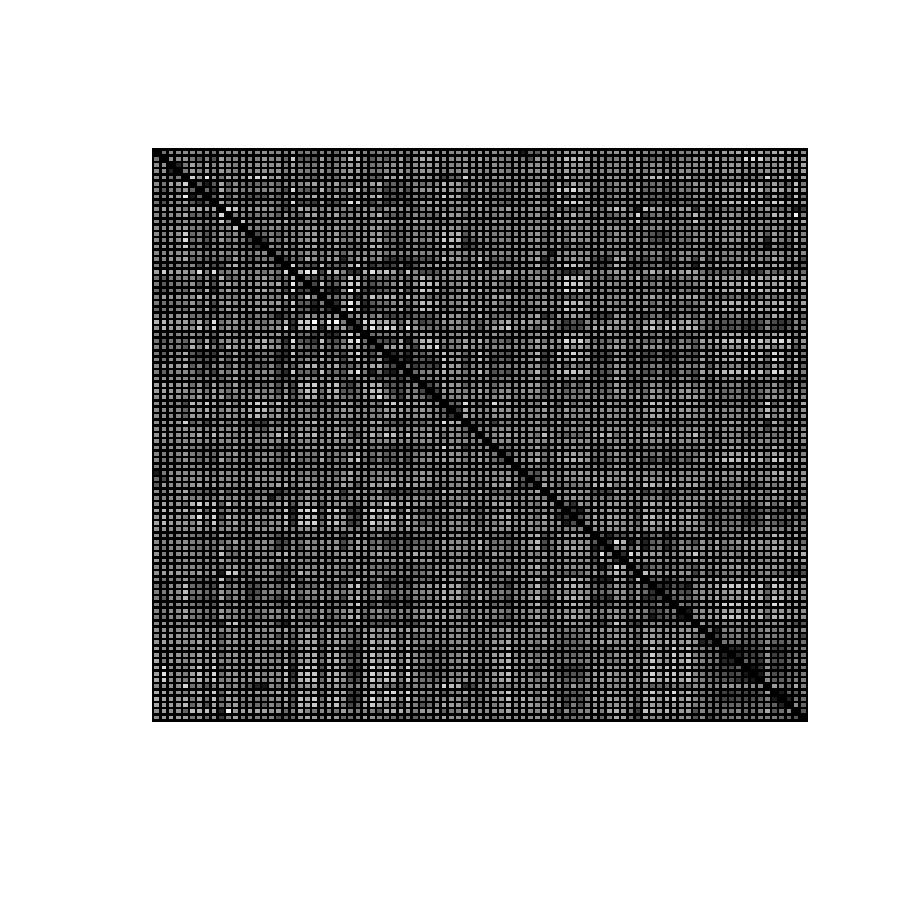
\includegraphics[width=5in]{memoria-autoc_clean}
\caption{Autocorrelació de les 88 variables.} \label{fig:_clean}
\end{figure}
\end{center}

%%%%%%%%%%%%%%%%%%%%%%%%%%%%%%%%%%%%%%%%%%%%%%%%%%%%%%%%%%%%%%%%%%%%%%%%%%%%%%%%%%%%%%%%%%%%%%%%%%%
\section{Reducció de dimensionalitat}

%%%%%%%%%%%%%%%%%%%%%%%%%%%%%%%%%%%%%%%%%%%%%%%%%%%%%%%%%%%%%%%%%%%%%%%%%%%%%%%%%%%%%%%%%%%%%%%%%%%
\section{Classificadors}
\subsection{LDA, QDA}
\subsection{k-NN}
\subsection{SVM}
\subsection{Xarxes Neuronals}
\subsection{Arbres}
\subsection{Random Forest (opcional)}
\subsection{Unió de classificadors}
%%%%%%%%%%%%%%%%%%%%%%%%%%%%%%%%%%%%%%%%%%%%%%%%%%%%%%%%%%%%%%%%%%%%%%%%%%%%%%%%%%%%%%%%%%%%%%%%%%%
\section{Conclusions}

%%%%%%%%%%%%%%%%%%%%%%%%%%%%%%%%%%%%%%%%%%%%%%%%%%%%%%%%%%%%%%%%%%%%%%%%%%%%%%%%%%%%%%%%%%%%%%%%%%%

\appendix
\section{Primer Apèndix}

%%%%%%%%%%%%%%%%%%%%%%%%%%%%%%%%%%%%%%%%%%%%%%%%%%%%%%%%%%%%%%%%%%%%%%%%%%%%%%%%%%%%%%%%%%%%%%%%%%%
\begin{thebibliography}{9}


\bibitem{strimmer10}
  Miika Ahdesmaki and Korbinian Strimmer,
  \emph{Feature selection in omics prediction problems using CAT scores and False Nondiscovery Rate Control},
  The Annals of Applied Statistics, 
  Vol. 4,
  2010.


\end{thebibliography}

\end{document}
